\subsection{Deep Learning}
Deep learning is a branch of machine learning. The main difference between the use of machine learning and deep learning, is that machine learning is not suitable for handling raw data form. Instead a machine learning system often needs a feature extractor, that will generate a feature vector from the data that can be used as an input for the machine learning system.
Deep learning is based on different techniques that makes it able to handle that data in its raw form, mainly because of its structure.\citep{LeCun2015, Schmidhuber2015} Because of this the system will automatically detect the necessary representations needed for classification and detection. Neural network is a structure of deep learning which consists of different layers, that can be divided into a input-layer and an output-layer, with one or more hidden layers in between \citep{Schmidhuber2015}. The key aspect of these layers is that the features are not defined by programmers, but they are found and learned from raw data using a general–purpose learning procedure.\citep{LeCun2015} An example of a neural network structure can be seen in figure \ref{fig:NN_structure}.   

\begin{figure} [H]
\centering
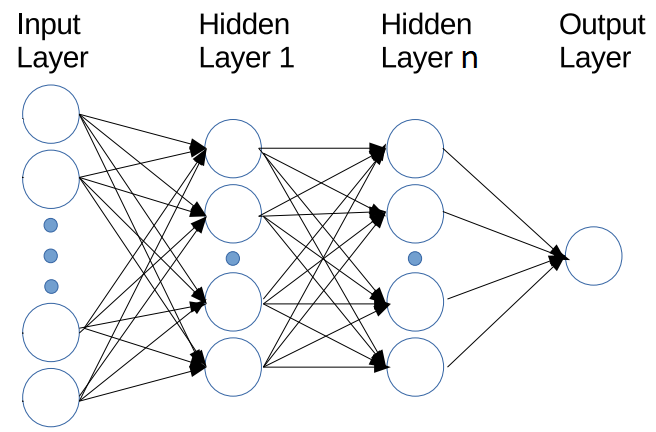
\includegraphics[width=0.6\textwidth]{figures/NN_structure}
\caption{Example of the neural network with possible layers\citep{Acquarelli2017}.}
\label{fig:NN_structure}  
\end{figure}

\noindent
The different layers consist of a series of nodes, where each node is connected by weights to one or several other nodes from a different layer. In the input-layer the nodes receive data. The second layer will then receive the output from the previous layer, and this process continues through the layers until the output-layer is reached.\citep{Schmidhuber2015} An example of how the hidden layers affect an image can be explained as follows:  
Firstly, the system detects minor changes like edges. Secondly, the edges are compared and put together to make up different kind of shapes. In the third hidden layer, it will be further combined to make up an object that can be identified.\citep{LeCun2015}

%Maybe explain a bit more to how the different nodes contain activation functions...

% Maybe explain how the input becomes the output in a litte more detail.  The weights are interconnection between two layers and they work as a set of coefficients, defining an image feature.\citep{Hameed2016}

% The following is already discriped in back prop, but could be used earlier or later maybe - By adjusting weights in the neural network it is possible to fit the model better to the training data, and thereby increase its accuracy and reduce error \citep{LeCun2015}.

\subsubsection{Learning scenarios}
There are different approaches for training a neural network, where the three main learning scenarios are supervised and unsupervised learning.

\noindent
\textbf{Supervised learning} is the most common way of training in machine learning. When applying this learning method the neural network is trained with input data that has a corresponding label. The network calculates an output through the forward pass, where the data is simply passed through the network. This output may then be compared to the label, and used to evaluate the performance of the system. As a result of the evaluation, the network may learn form the data by doing a backward pass through the network, also known as backpropagation. \citep{LeCun2015} Overall supervised learning may be described as teaching the network how to associate a given input to a specific output \citep{Goodfellow0216}, and is mostly associated with classification, regression, and ranking problems \citep{Mehryar2012}.

\noindent
\textbf{Unsupervised learning} is when training i performed with data that has no output label. Instead of learning associations between input and output, the network organizes the data by searching for common characteristics \citep{Mehryar2012}. An example of an unsupervised learning algorithm is k-mean clustering, where the unlabeled dataset goes through a classification, and splits data into clusters that are near each other \citep{Goodfellow2016}.  

%\noindent
%\textbf{Semi-supervised learning} network receives both labeled, unlabeled data and then it searches for common characteristics in data. It is used mainly when the labeled data is hardly collected and unlabeled data is easily reachable. \citep{Mehryar2012}

  
\subsection{Back-propagation}
Backpropagation is a popular learning algorithm in neural networks, that is based on gradient decent, and used because of it's simplicity and computationally efficiency. \citep{Bengio2012, Duda2000}
It's the (learning) process where the weights of a neural network are adjusted in order to reduce the error calculated between the output of the network and the expected output. This by definition makes backpropagation closely related to supervised learning, as written in \ref{sec:LearningTech}, to which backpropagation the most general method used.\citep{Duda2000}  
When a neural network is initialized the weight may be set with a random value, meaning that the neural network may perform very poorly through the first iterations of training. Based on a cost function a loss is calculated for every input that passes through the network, the is used by backpropagation to make the adjustments on the weight to reduce this loss. As training progresses the loss should decrease as a result of the weight adjustments, and improve the performance of the neural network. \citep{LeCun2015, Duda2000, Goodfellow2016}   
This learning process continues until optimal weights with minimum error is reached.\citep{Hameed2016}

The basic idea behind it is to minimize the overall output error as much as possible during the learning stage. This algorithm process is divided in two main stages: forward and backward. In the first process (forward), the back-propagation architecture is described as  the inputs and weights multiplication of each node (separate input) summed with additional coefficients called biases.\citep{Hameed2016} 

MAYBE TALK ABOUT ACTIVATION FUNCTIONS IN RELATION TO BACKPROPAGATION. 

A PROBLEM OFTEN RELATED TO OPTIMIZATION IS THE LAGER THE NETWORK THE HARDER IT IS TO OPTIMIZE, BUT IN ANOTHER WAY IF THE NETWORK IS SMALL AND SIMPLE THE EASIER IT IS TO OPTIMIZE. 

\subsubsection{Gradient Decent, mini-batches and optimizers}

% Mention local minima and gobal minima and why it is not so importent to find the absolut global minima \citep{Duda2000}. 

% Mention the mini bacthes are used in order to reduce the computation cost, and that the size of the mini-batch is often what limits the network computation. 



\subsubsection{Learning curves}
During the beginning of training, the training error of network will typically be relatively high, but during training the error decreases monotonically, as the weights are adjusted in the network \citep{Duda2000}. An illustration of how the error values are affected during training can be seen in \autoref{fig:learningCurve}.

\begin{figure} [H]
\centering
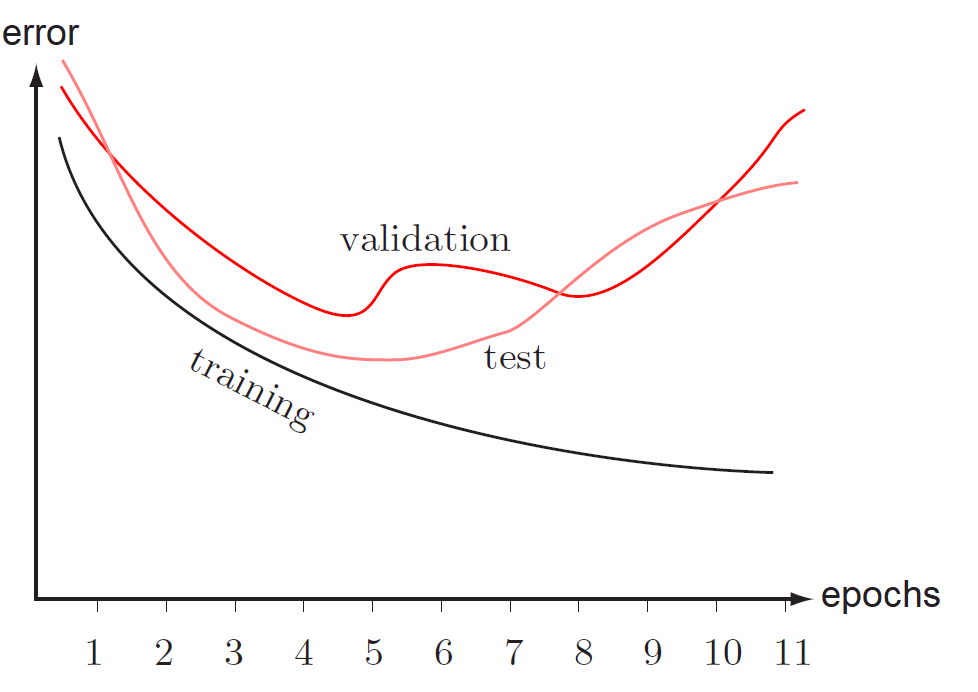
\includegraphics[width=0.7\textwidth]{figures/learningCurves}
\caption{Illustration of how training (black), validation (red), and test (orange) error is affected by the increase in epochs. Edited from \citep{Duda2000}.}
\label{fig:learningCurve}
\end{figure}

From the figure it can be seen how the error value of the validation, can be used to evaluate the network. 
Near the fifth epoch the validation and the test error starts to rise, indicating that the network is overfitting to the training data, thereby decreasing the generalization abilities. 
Validation error can therefor be used as stop criterion for when the training is optimal, and prevent overfitting. 
Typically the validation and test error will always be higher that the training error, which is also seen in \autoref{fig:learningCurve}. \citep{Duda2000}


\subsection{Core NN layers}
\subsubsection{Convolutional Neural Networks}
Convolutional neural networks (CNNs) perform highly in several tasks, including digit recognition, image classification and face recognition. The key aspect of CNNs is to automatically learn a complex model by extracting visual features from the pixel-level content.
CNNs are feed–forward models that map input data with a set of suitable outputs. 
Accuracy and performance rely on large training datasets and training procedure based on back-propagation with optimization algorithm such as gradient descent which is used for finding minimum value of the function.\citep{Acquarelli2017}

What is convolution. 
Convolutional Neural Networks (CNNs) a type of special neural network for processing data with a grid-like topology \citep{Goodfellow2016}. 

Convolution is almost always combined with a pooling layer \citep{Goodfellow2016}, and is also known as the typical architecture of a convolutional neural network \citep{LeCun2015}.  

The terminology regarding the output of a convolutional layer can be refered to as a feature map \citep{Goodfellow2016} 




